\documentclass{article}
\usepackage[utf8]{inputenc}
\usepackage{polski}
\usepackage{geometry}
\usepackage{pdfpages}
\usepackage{pdfpages}
\usepackage{listings}

\geometry{
a4paper,
total={170mm,257mm},
left=20mm,
top=20mm
}
\renewcommand\thesection{}

\title{Podstawy baz danych\\ Projekt konferencje}
\author{Agnieszka Dutka, Maciek Trątnowiecki}
\date{AGH, Styczeń 2020}

\begin{document}
\maketitle
\section{Objaśnienie schematu bazy}
        \begin{itemize}
            \item Clients - Reprezentuje klientów chcących opłacić miejsca na konferencjach i warsztatach. Klientem może być zarówno firma, jak i osoba prywatna. W zależności od tego dane klienta reprezentowane są przez odpowiednią relację w bazie. 
            
            \item Companies - Jeśli klient jest firmą, przechowuje jego dane. 
            
            \item Participants - Jeśli klient jest osobą prywatną, przechowuje jego dane.
            
            \item Conferences - Reprezentuje konferencję z którą powiązane są odpowiednie dni konferencyjne, oraz warsztaty. 
            
            \item Conference\_days - Reprezentuje pojedynczy dzień konferencji. Powiązana jest z nim ustalona opłata za uczestnictwo. Zniżki obowiązujące w zależności od daty rejestracji zwarte są w relacji Early\_Signup\_Discounts. 
            
            \item Early\_Signup\_Discounts - Odpowiada za informację o tabeli zniżek na dany dzień konferencyjny. Pojedyncza zniżka przechowywana jest w krotce z atrybutami w postaci procentowej obniżki ceny standardowej, oraz ostatniego dnia w którym obowiązuje. 
            
            \item Conference\_day\_reservations - Realizuje rezerwacje na poszczególny dzień konferencji. Każda rezerwacja powiązana jest z klientem, który ją opłaca. Za powiązanie rezerwacji z uczestnikiem odpowiada osobna relacja. Zawiera także pole due\_price określające termin płatności. Atrybut active odpowiada za możliwość rezygnacji z podjętej rezerwacji (uznaliśmy, że usuwanie krotki z bazy może nie być optymalnym rozwiązaniem, jako że zawarte w niej dane mogą jeszcze być przydatne z punktu widzenia logiki biznesowej). Atrybuty adult\_seats i student\_seats służą do liczenia kosztu podjęcia rezerwacji przed powiązaniem jej z uczestnikami konferencji. 
            
            \item Conference\_day\_registration - Wiąże rezerwację z uczestnikami konferencji. Atrybut is\_student informuje, czy danemu uczestnikowi przysługuje zniżka studencka. 
            
            \item Payments - Przechowuje informacje o wpływach pieniężnych powiązanych z daną rejestracją. 
            
            \item Workshops - Reprezentuje warsztaty odbywające się w trakcie odpowiednich dni konferencyjnych.
            
            \item Workshops\_reservations - Opisuje rezerwacje na warsztaty w sposób analogiczny do rezerwacji na konferencje. 
            
            \item Workshops\_registrations - Łączy rezerwację z uczestnikami w sposób analogiczny do dni konferencyjnych.
            
        \end{itemize}
    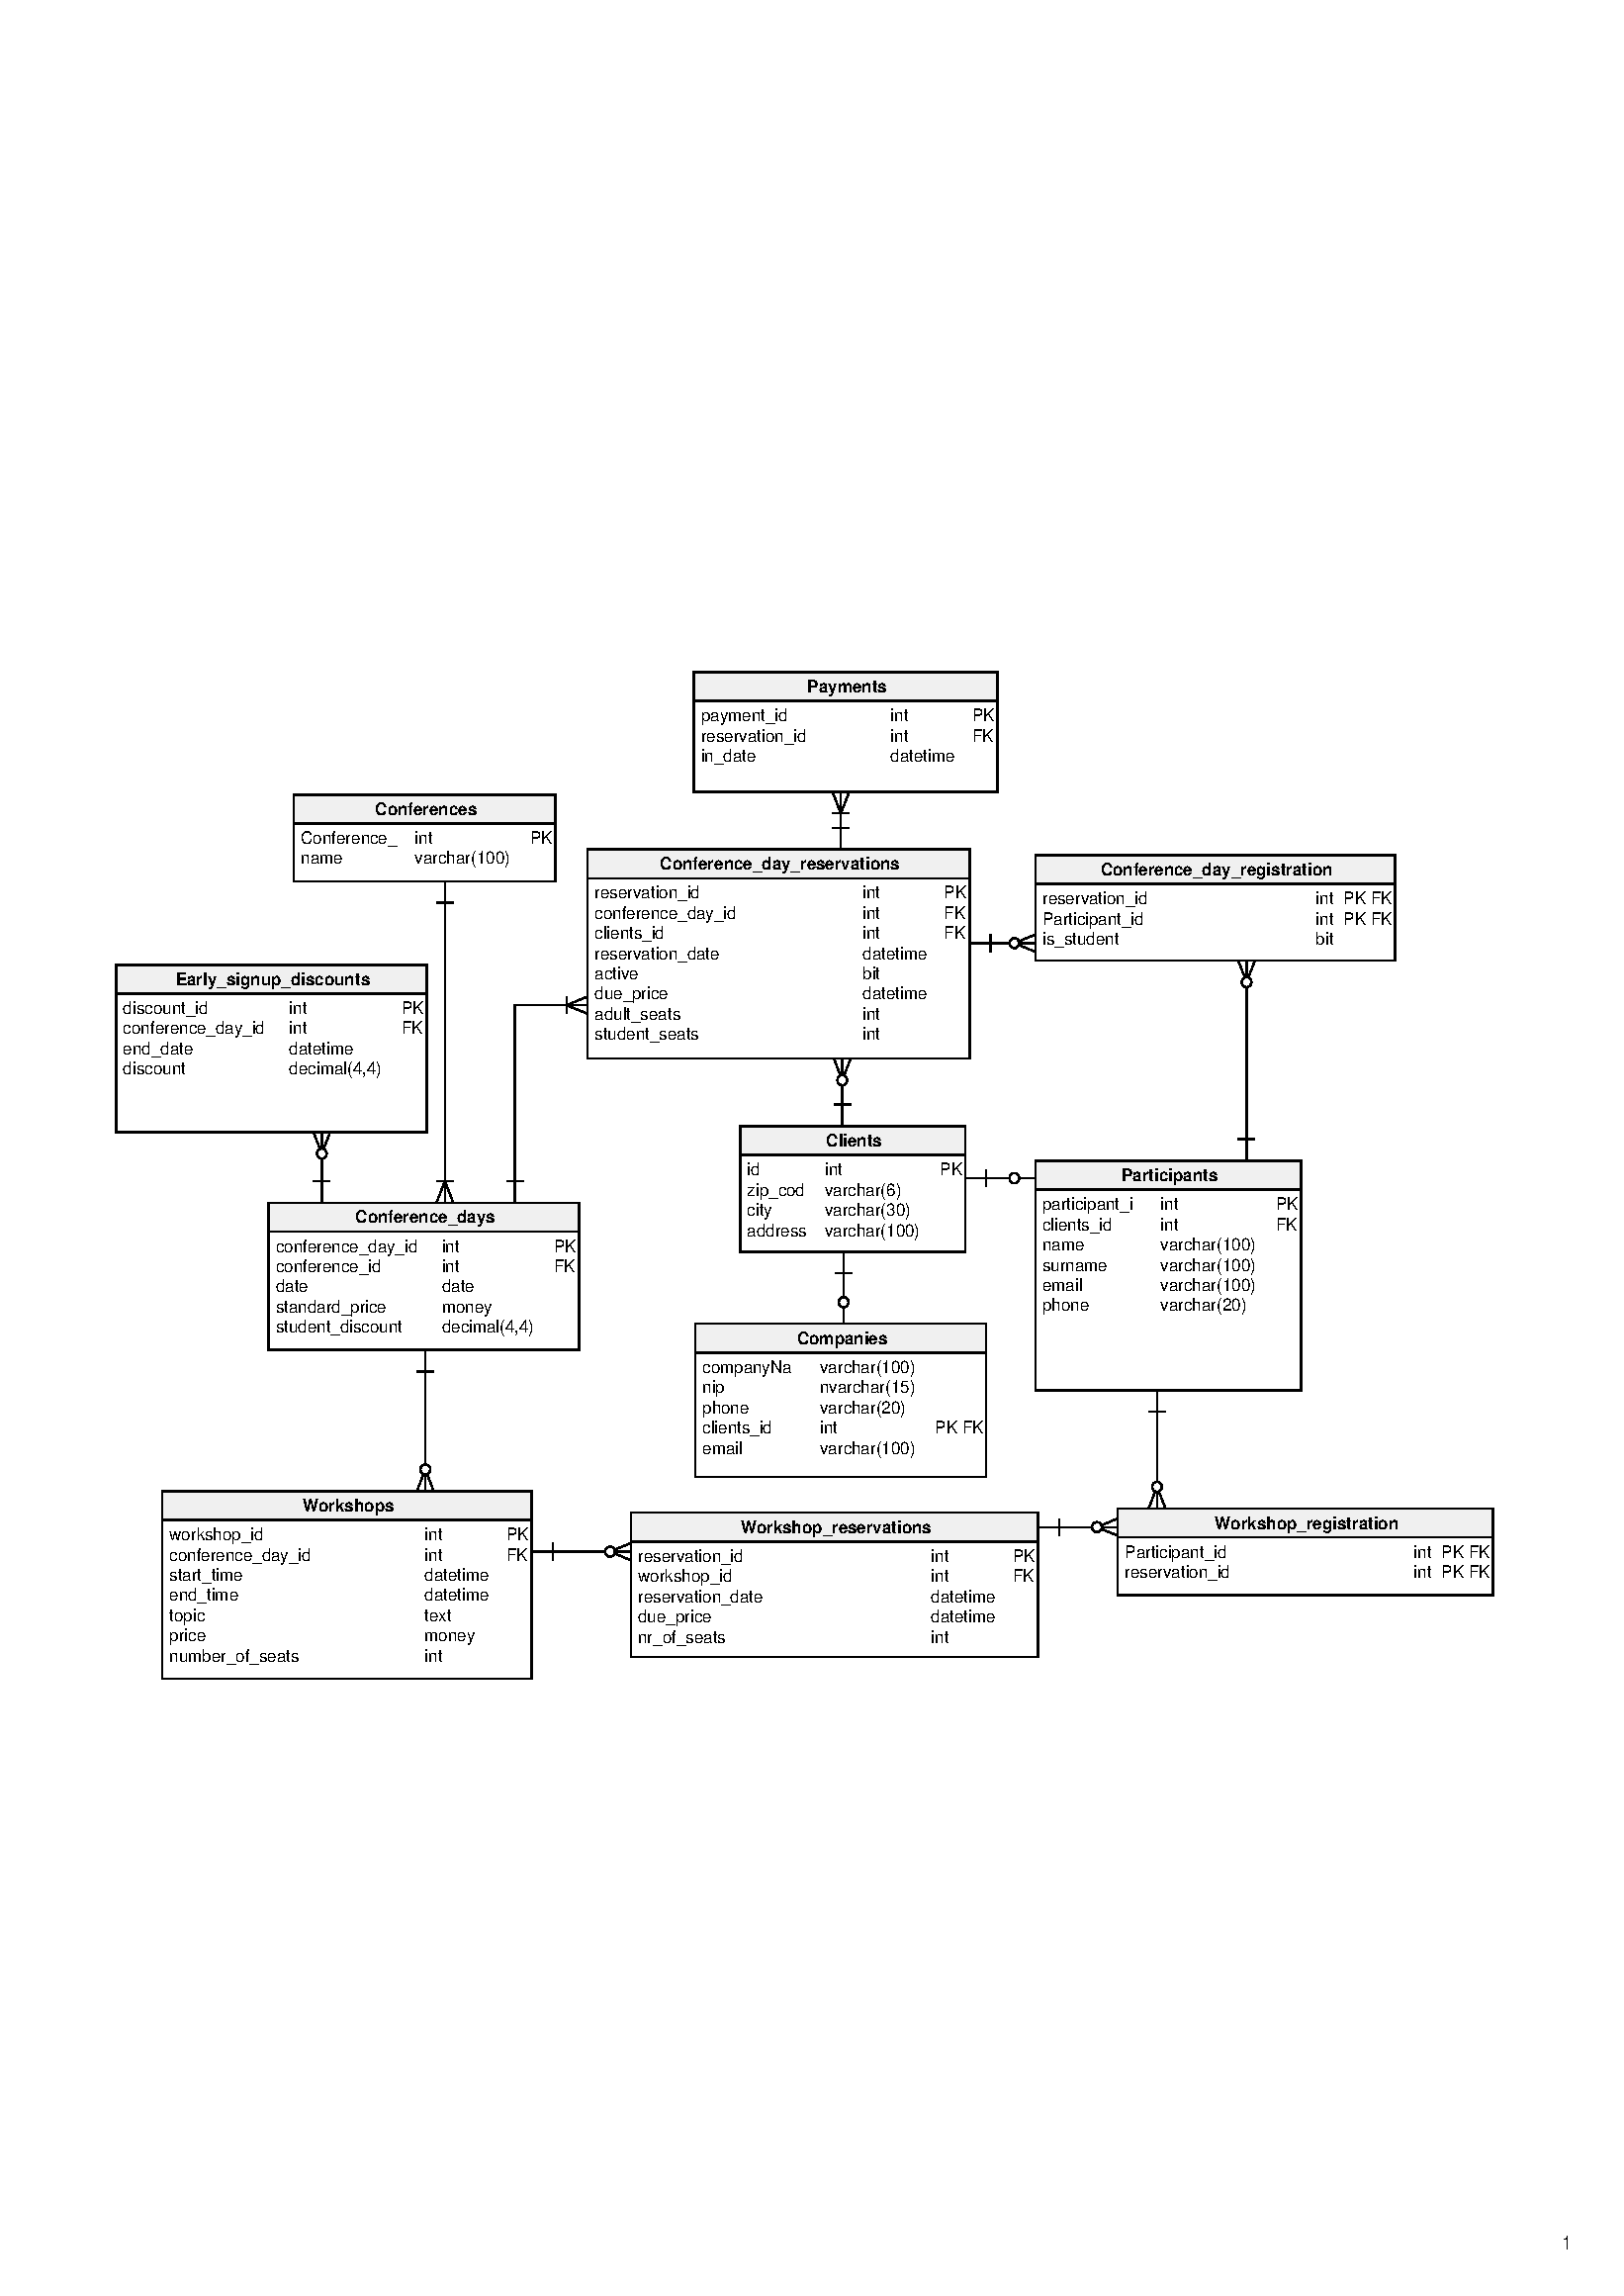
\includepdf{../Diagrams/Scheme.pdf}    
    
\lstset{ 
  backgroundcolor=\color{white},   % choose the background color; you must add \usepackage{color} or \usepackage{xcolor}; should come as last argument
  basicstyle=\footnotesize,        % the size of the fonts that are used for the code
  breakatwhitespace=false,         % sets if automatic breaks should only happen at whitespace
  breaklines=true,                 % sets automatic line breaking
  captionpos=b,                    % sets the caption-position to bottom
  commentstyle=\color{mygreen},    % comment style
  deletekeywords={...},            % if you want to delete keywords from the given language
  escapeinside={\%*}{*)},          % if you want to add LaTeX within your code
  extendedchars=true,              % lets you use non-ASCII characters; for 8-bits encodings only, does not work with UTF-8
  firstnumber=1000,                % start line enumeration with line 1000
  frame=single,	                   % adds a frame around the code
  keepspaces=true,                 % keeps spaces in text, useful for keeping indentation of code (possibly needs columns=flexible)
  keywordstyle=\color{blue},       % keyword style
  language=Octave,                 % the language of the code
  morekeywords={*,...},            % if you want to add more keywords to the set
  numbers=left,                    % where to put the line-numbers; possible values are (none, left, right)
  numbersep=5pt,                   % how far the line-numbers are from the code
  numberstyle=\tiny\color{mygray}, % the style that is used for the line-numbers
  rulecolor=\color{black},         % if not set, the frame-color may be changed on line-breaks within not-black text (e.g. comments (green here))
  showspaces=false,                % show spaces everywhere adding particular underscores; it overrides 'showstringspaces'
  showstringspaces=false,          % underline spaces within strings only
  showtabs=false,                  % show tabs within strings adding particular underscores
  stepnumber=2,                    % the step between two line-numbers. If it's 1, each line will be numbered
  stringstyle=\color{mymauve},     % string literal style
  tabsize=2,	                   % sets default tabsize to 2 spaces
  title=\lstname                   % show the filename of files included with \lstinputlisting; also try caption instead of title
}

\section{Implementacja}
    \lstinputlisting[language=sql]{../Create.sql}
    \newpage

\newpage 
\section{Widoki}
    \lstinputlisting[language=sql]{../Views/Views.sql}
    
\newpage 
\section{Funkcje}
Funkcja sprawdzająca czy wprowadzony NIP jest zgodny z obowiązującymi prawami.
    \lstinputlisting[language=sql]{../Functions/isValidNip.sql} \newline
Funkcja sprawdzająca czy dany klient jest firmą. 
    \lstinputlisting[language=sql]{../Functions/isClientCompany.sql} \newline
Funkcja zwracająca imię i nazwisko klienta (jeśli jest on osobą fizyczną).
    \lstinputlisting[language=sql]{../Functions/showClientsName.sql} \newline
Funkcja zwracająca ilość wolnych miejsc na danej konferencji.
    \lstinputlisting[language=sql]{../Functions/FreeSeats/conferenceFreeSeats.sql} \newline
Funkcja zwracająca ilość wolnych miejsc na danych warsztatach.
    \lstinputlisting[language=sql]{../Functions/FreeSeats/workshopFreeSeats.sql} \newline
Funkcja zwracająca imiona i nazwiska uczestników danej konferencji.
    \lstinputlisting[language=sql]{../Functions/ParticipantsLists/participantsForGivenConference.sql} \newline
Funkcja zwracająca imiona i nazwiska uczestników danego warsztatu.
    \lstinputlisting[language=sql]{../Functions/ParticipantsLists/participantsForGivenWorkshop.sql} \newline
Funkcja zwracająca całkowity balans danego klienta.
    \lstinputlisting[language=sql]{../Functions/PaymentsAndPrices/clientsBalance.sql} \newline
Funkcja zwracająca koszt danej rezerwacji na dzień konferencji (łącznie z ceną podpiętych warsztatów).
    \lstinputlisting[language=sql]{../Functions/PaymentsAndPrices/confDayPrice.sql} \newline
Funkcja zwracająca dotychczasowo wpłaconą kwotę na daną rezerwację.
    \lstinputlisting[language=sql]{../Functions/PaymentsAndPrices/confReservationPaidAmount.sql} \newline
Funkcja zwracająca koszt danej rezerwacji na warsztaty.
    \lstinputlisting[language=sql]{../Functions/PaymentsAndPrices/confReservationPrice.sql} \newline

\newpage
\section{Procedury}
Procedury służące wprowadzaniu nowych danych do bazy:
    \lstinputlisting[language=sql]{../Procedures/AdditionProcedures.sql}
Procedury usuwające dane z bazy:
    \lstinputlisting[language=sql]{../Procedures/DeleteProcedures.sql}
Procedury aktualizujące informacje zawarte w bazie danych:
    \lstinputlisting[language=sql]{../Procedures/UpdateProcedures.sql}

\newpage
\section{Generator danych}
    \lstinputlisting[language=python]{../Generator/main.py}
    \lstinputlisting[language=python]{../Generator/AbstractClass.py}
    \lstinputlisting[language=python]{../Generator/AbstractGenerator.py}
    \lstinputlisting[language=python]{../Generator/Client.py}
    \lstinputlisting[language=python]{../Generator/ClientsGenerator.py}
    \lstinputlisting[language=python]{../Generator/Company.py}
    \lstinputlisting[language=python]{../Generator/ConfDayReservation.py}
    \lstinputlisting[language=python]{../Generator/ConfDayResGenerator.py}
    \lstinputlisting[language=python]{../Generator/ConfDaysGenerator.py}
    \lstinputlisting[language=python]{../Generator/ConferenceDay.py}
    \lstinputlisting[language=python]{../Generator/ConferenceGenerator.py}
    \lstinputlisting[language=python]{../Generator/Conference.py}
    \lstinputlisting[language=python]{../Generator/ConfRegistrationGen.py}
    \lstinputlisting[language=python]{../Generator/ConfRegistration.py}
    \lstinputlisting[language=python]{../Generator/EsdGenerator.py}
    \lstinputlisting[language=python]{../Generator/Esd.py}
    \lstinputlisting[language=python]{../Generator/Participant.py}
    \lstinputlisting[language=python]{../Generator/ParticipantsGenerator.py}
    \lstinputlisting[language=python]{../Generator/PaymentGen.py}
    \lstinputlisting[language=python]{../Generator/Payment.py}
    \lstinputlisting[language=python]{../Generator/WorkshopGenerator.py}
    \lstinputlisting[language=python]{../Generator/Workshop.py}
    \lstinputlisting[language=python]{../Generator/WorkshopRegistrationGen.py}
    \lstinputlisting[language=python]{../Generator/WorkshopRegistration.py}
    \lstinputlisting[language=python]{../Generator/WorkshopResGen.py}
    \lstinputlisting[language=python]{../Generator/WorkshopRes.py}

\newpage
\section{Uprawnienia}
    \begin{enumerate}
        \item Administrator - Całkowity dostęp do bazy.
        \item Pracownik – Dostęp poziomu organizatora dla wszystkich konferencji. 
        \item Organizator – Dostęp do wszystkich rekordów powiązanych z konkretną konferencją. Możliwość edycji tabel warsztatów, dni konferencyjnych.  
        \item Klient – Rejestracja na konferencje i warsztaty, wprowadzanie danych osobowych.
        \item Uczestnik – Wgląd  i edycja wprowadzonych danych osobowych, podgląd warsztatów  i dni konferencyjnych na jakie jest zapisany (nie może generować kosztów, jako że jest podpięty pod klienta). 
    \end{enumerate}
\end{document}
